\section{Language and system overview}
\label{sect:Overview}
In this section, we give an overview of the system architecture within which \rolang programs execute and then discuss key language features with an example.

We call an entity executing a \rolang program an {\em agent\/} or a {\em process.\/}
The hardware abstraction on which \rolang programs executes includes (a) a controller, (b) shared memory, in addition to the usual (c) local memory and processing unit of the agent.  
%
The controller receives lists of way-points and obstacles from the agent's program, drives the actuators (e.g. motors) to reach the way-points while avoiding the obstacles using sensors (e.g. GPS), and updates certain flags to indicate its status to the program.
%
The shared memory abstraction provides single-writer and multi-writer distributed shared variables using which an agent's program can communicate with another agent's program. 

%A \rolang program interacts with 
\begin{figure}[t!]
	\centering
	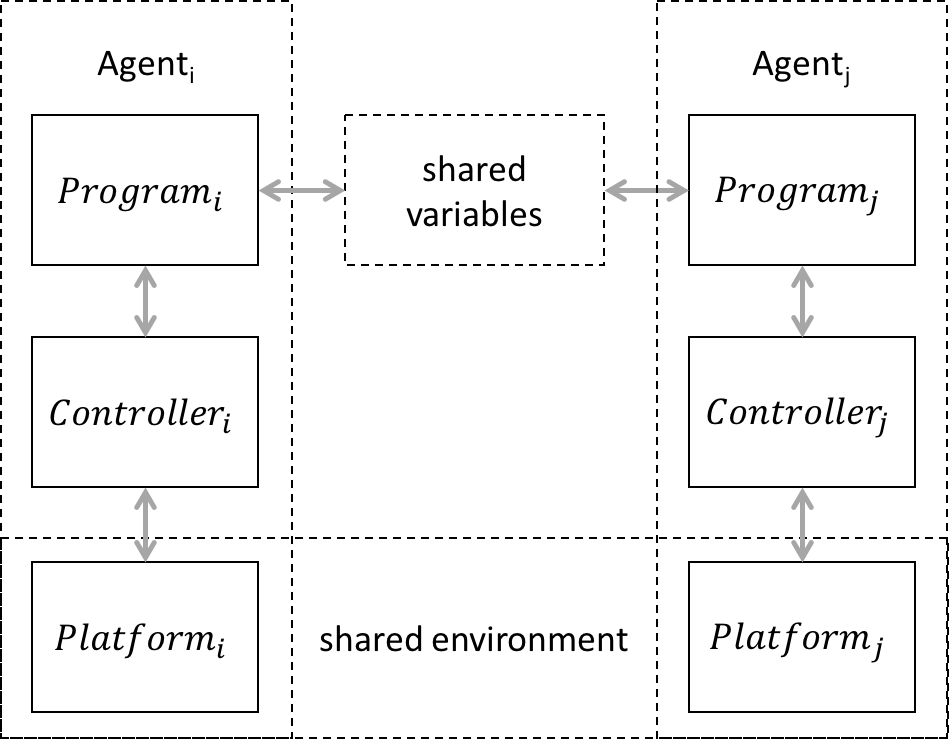
\includegraphics[scale=0.4]{figs/arch.png}
	\caption{\small Architecture of distributed system. Agent programs interact through shared variables. Each agent program also sets waypoints for its own controller which control the physical motion of the agent's platform. The agent platforms inhabit a shared physical environment, and therefore, also interact physically.}
	\label{fig:arch}
\end{figure}

%\rolang allows users to write applications that will run on a distributed system of agents. 
For this paper, we assume that all agents execute the same \rolang program; each agent knows the IDs of all participants; and there is a common coordinate system for the physical space within which the agents are operating. 
%
A program is a collection of \emph{variable declarations} and \emph{events}. 
The language provides two types of shared variables:
(a) a {\em multi-writer} shared variable $x$ is declared as $\MW$ and allows all agents to do reads and writes on $x$. 
(b) a {\em single-writer\/} shared variable $x$ is declared as $\SW$ block, and it 
creates an array $x\langle \cdot \rangle$ 
where the $i^{th}$ component $x \langle i \rangle$ can be read by all but can only be written to by agent $i$.
%Local variables are declared in \verb|Loc|al declaration blocks.  \newline

A \rolang program is organized as a collection of events. Each event nominally has a precondition (or guard) and an effect. The effect is a sequence of program statements and it may be executed only when the precondition holds. An event is said to be enabled if its precondition holds. If multiple events of a given agent program are enabled, then any one of them is chosen.  
%
%
% The \verb|EventBlock| can be seen as a (potentially) infinite while-loop. 
%
%
There is a special event called \verb|Init|
that is executed when the program starts. 
% event, and an \verb|EventBlock|. The \verb|Init| event occurs at the beginning when the application starts executing, and it contains all statements which need to be executed only once; for instance, initializing a shared array. After the \verb|Init| event is executed, the \verb|EventBlock| starts executing. 
 
\rolang provides a special operation \verb|doReach| for programs to interact with the agent's controller (see Figure~\ref{fig:arch}). 
A call to \verb|doReach| instructs the controller to move towards a \emph{target} (position or configuration) while avoiding a set of \emph{obstacles}---both specified in the common coordinate system. Successive calls to \verb|doReach| may update the sequence of targets and obstacles. 
%
The controller communicates with the program using two flags: (a) \emph{doReach_done} is set if a neighborhood of the target is reached, and (b)\emph{doReach_fail} is set if the controller determined that it cannot reach the target while avoiding the obstacles. 
%
\sayan{Why different font for the flags? Use the same macros/conventions as in the code fragment.}
%
Implementations of  controllers for different kinds of agents platforms (e.g., ground rovers and quadcopters) provide different  best-effort strategies. 
\sayan{In defining the semantics of \rolang the controller is treated as a parameter (see Section~\ref{missing}). Need to sharpen this statement.}

% which need to be avoided. We do not need to specify the format of the obstacles, as different implementations of this \verb|doReach| can have different specifications, but the target in general has the same type as the time varying variables of the system. \verb|doReach| 
 
%The next section presents the formal syntax, and an example to illustrate the structure of a general application. 

 \subsection[h]{An Illustrative Example}
\label{sect:Eg}
We present a simple illustrative example to demonstrate some of the features of the language, and to aid discussion in future sections. We want to design an application where (a group of) robots try to visit a predetermined sequence of waypoints, with predetermined obstacles. We aim to ensure that a robot choosing the next destination will not pick a waypoint that has already been visited by some robot. The code for this application is provided in \reffig{Race}.

\lstset{basicstyle=\scriptsize\ttfamily,breaklines=false}

\begin{figure}[ht!]
\label{fig:Race}
\noindent\begin{minipage}{.5\textwidth}

\begin{lstlisting}
Agent::Race

allwrite:
	List<ItemPosition> dests 
    	= getInput();
allread:

loc:
  ObstacleList obs = getObs();
  boolean Pick = true; 
  ItemPosition currentDest;
Init:

PickDest():
  pre(Pick);
  eff:
    if (isEmpty(dests)):
    exit();   
 \end{lstlisting}
 \end{minipage}\hfill
\noindent\begin{minipage}{.5\textwidth}

\begin{lstlisting}
    else:
      currentDest = head(dests);
      doReach(currentDest,obs);
      Pick = false;
      
Remove():
  pre(!Pick);
  eff:
    if(doReach_done):
      atomic:
        if(contains(
        dests,currentDest)):
        remove(dests,currentDest);
   	  Pick = true;
 \end{lstlisting}
 \end{minipage}\hfill
 \caption{Race Application}
 \end{figure}
\verb|ItemPosition| is a built-in datatype which is used to represent the position of the robot (the physical coordinates $(x,y,z)$). The robots have a shared list of \verb|ItemPosition|s (\verb|dests|) which is initialized using the built-in function \verb|getInput|. We define a boolean variable \verb|Pick| which determines whether the robots are in the stage of picking and moving to the current destination (\verb|currentDest|), or removing the current destination from the shared list of destinations, since it was visited. Functions such as \verb|getInput()|, \verb|getObs()| are provided as uninterpreted functions, which can be defined in an external language as long as they return values with consistent types. \footnote{Changing this line}

 The first stage is \verb|PickDest|, when the next destination in the race is set, the robots try to reach it while avoiding the provided obstacles. Then in the \verb|Remove| stage, each robot \emph{atomically} updates the list of destinations to be visited if it reached the current destination. The \verb|atomic| construct ensures mutual exclusion while updating a shared variable. The function \verb|remove| can only remove an item from a list if it contains said item, the execution gets stuck otherwise. With that in mind, we added a check for whether the \verb|currentDest| is contained in \verb|dests| \emph{within} the atomic block; to ensure that between this check and atomically trying to remove the list element, another robot didn't successfully already remove the same element. 